\fancyhead[L]{Guide Utilisateur}
\fancyhead[C]{Overlays durant la partie}

\label{sec:overlays}
\section{Overlays durant la partie}
\subsection{Qu'est-ce que sont les overlay en jeu ?}
Palantir vous propose une stratégie de base qui change en fonction de la civilisation que vous aurez choisi. Celle-ci se mettra à jour en fonction de l'âge dans lequel vous êtes actuellement, vous donnant ainsi une stratégie base qui vous accompagne tout au long de votre partie pour vous aider à tenir les timings et les ressources bases pour profiter du jeu et avoir de la vraie compétition durant vos parties.

\subsection{Overlay de stratégie}
L'overlay de stratégie se base sur \hyperref[sec:configfiles]{\textbf{\textit{le fichier de configuration}}} de la civilisation sélectionnée pour vous afficher chaque étape de la stratégie à l'âge dans lequel vous vous trouvez actuellement. Vous pouvez naviguer facilement dans la stratégie grâce aux boutons présents sur l'interface.

\begin{figure}[ht!]
    \begin{center}
        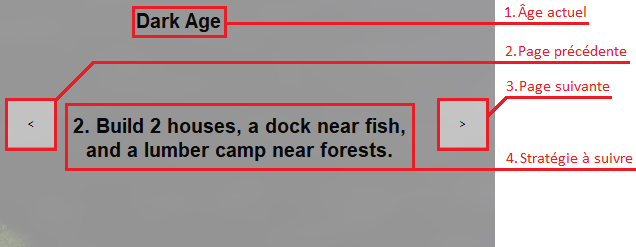
\includegraphics[scale = 0.87]{in-game-overlay.png}
    \end{center}
    \caption{Overlay de stratégie de base}
\end{figure}

\textbf{1.} Âge actuel : Âge actuel de votre civilisation.\\
\textbf{2.} Page précédente : Bouton allant à la page précédente de la stratégie.\\
\textbf{3.} Page suivante : Bouton allant à la page suivante de la stratégie.\\
\textbf{4.} Stratégie à suive : Descriptif de l'étape de la stratégie à suivre.

\newpage

\subsection{Overlay par seuils}
Cet overlay est aussi un des overlays qui s'afficheront durant la partie. Il ne s'affichera que lorsque certains seuils définis dans \hyperref[sec:configfiles]{\textbf{\textit{le fichier de configuration}}} seront atteint. Par exemple, il s'affichera si vous avez atteint le nombre de ressource nécessaire pour le passage de votre civilisation à l'âge suivant comme montré dans la Figure 4.

\begin{figure}[ht!]
    \begin{center}
        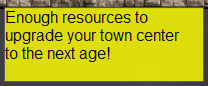
\includegraphics[scale = 0.87]{in-game-hint-overlay.png}
    \end{center}
    \caption{Overlay de seuil}
\end{figure}